\newsection
\subsection{Education}
\label{sec:education}
\sectionauthors{Ali Malik, Dorottya Demszky, Pang Wei Koh, Moussa Doumbouya, Drew A. Hudson, Allen Nie, Hamed Nilforoshan, Alex Tamkin, Emma Brunskill, Noah Goodman, Chris Piech}

\begin{figure}[!ht]
    \centering
    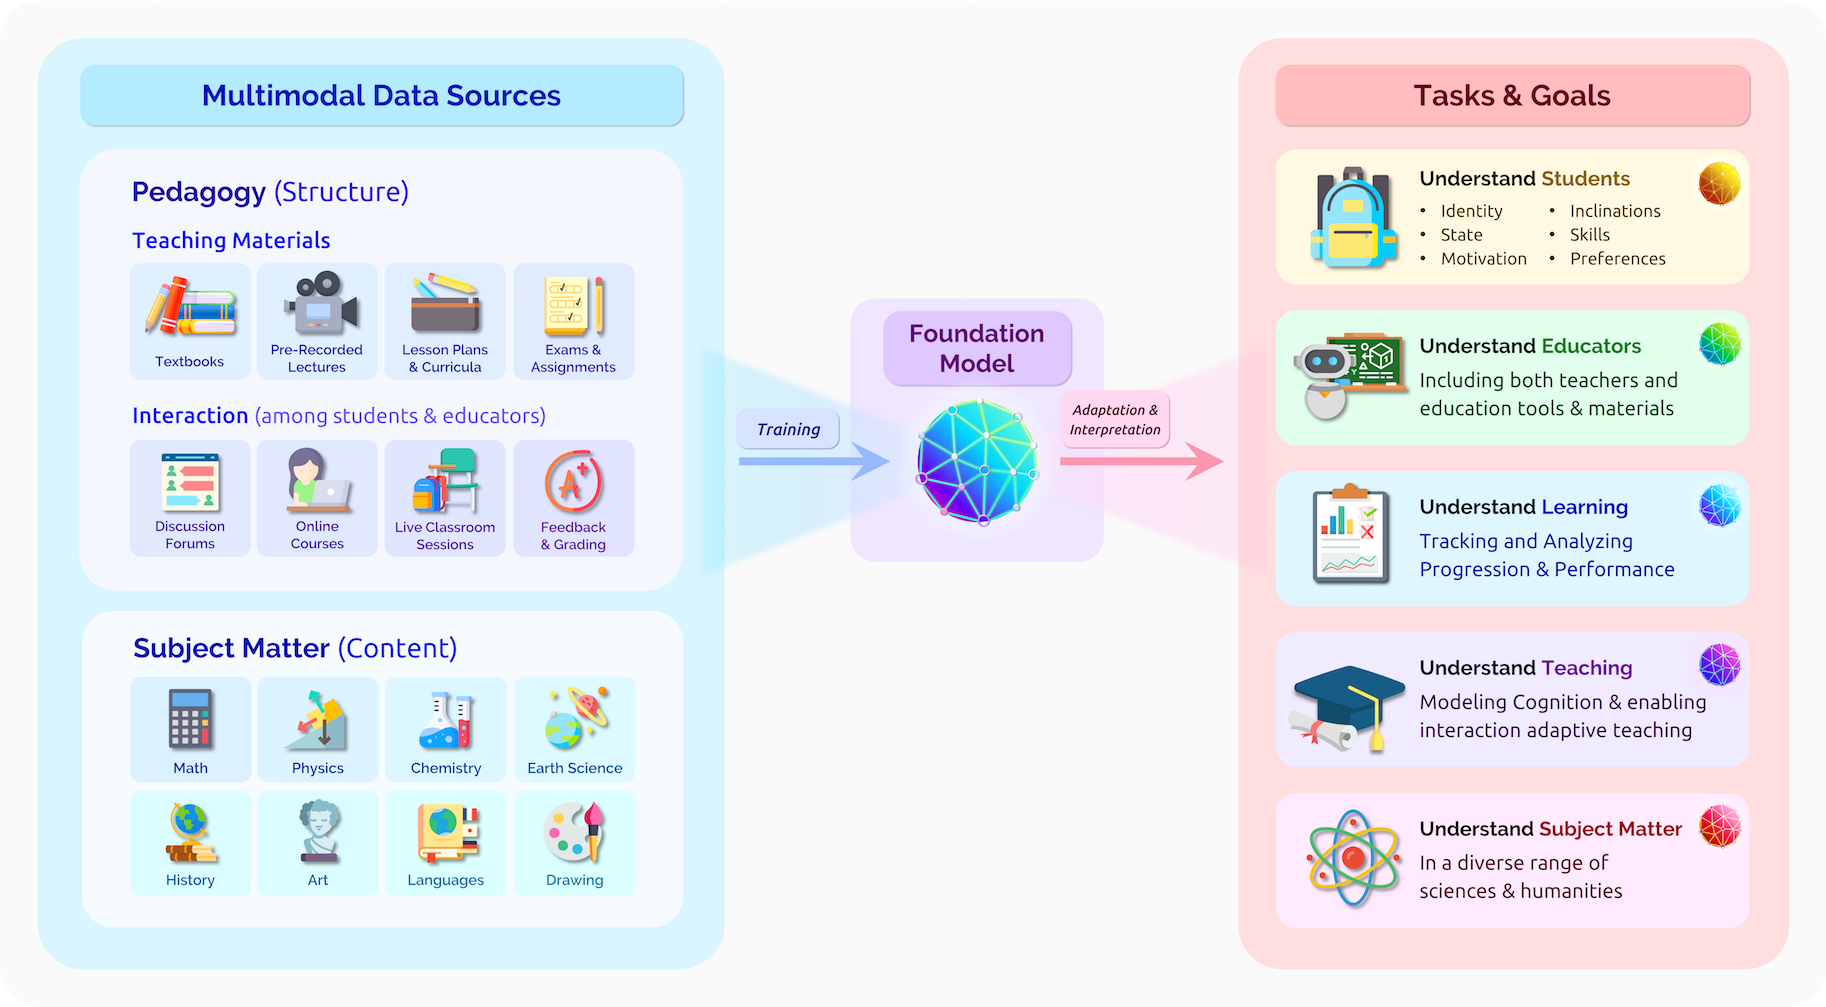
\includegraphics[width=\linewidth]{applications/education_figs/Education.png}
    \caption{Foundation models in education could be trained on multiple data sources to learn the capabilities necessary for education: an understanding of various subject matter and different pedagogical techniques. These foundation models can be applied in a general-purpose way across a range of tasks and goals such as understanding students, assisting teachers, and generating educational content.
    }
    \label{fig:education}
\end{figure}

In the year 2000, the largest gathering of world leaders convened at the United Nations Millennial Summit to reflect on an ideal vision for the future. Delegates concluded that a primary focus should be education, declaring it ``a foundation for human fulfillment, peace, sustainable development, economic growth, decent work, gender equality and responsible global citizenship."  This discussion was ultimately recodified into the United Nations Sustainable Development goal to ``ensure inclusive and quality education for all and promote lifelong learning" \cite{unsdg2015}.
% This expansive goal includes training for the next generation as well as reskilling workers who are trying to respond to  a rapidly changing job market, accelerated in part by advances in technology. 
However, providing high quality education at a large scale poses difficult societal and economic challenges. The price of education per student is growing faster than economy-wide costs \cite{bowen2012cost}, limiting the resources available to support student learning. 
In the United States, one symptom is that private education debt held by students has reached \$1.6 trillion, surpassing total credit card debt \cite{friedman2020debt}. Considering the rising need to provide adult retraining, the gap between the demand for education and our ability to provide it is alarmingly large. 

With the advent of the digital age and the rapid growth in digital learning,
computational approaches to education have shown promise in increasing the effectiveness of learners and teachers. Several core directions have emerged as potentially impactful applications of AI for education \cite{woolf2013aied}, such as systems that can provide meaningful feedback to students \cite{malik2021generative}, help teachers improve \cite{jensen2020toward, demszky2021measuring, suresh2021using}, or even create personalised and adaptive learning experiences that tailor the learning process to individual students' needs and dispositions \cite{connor2019using}. 

Despite this potential, computational education has proven to be exceptionally difficult. Existing work has focused on custom solutions to highly specific tasks for which large amounts of training data has to be collected from scratch. Due to the difficulty and cost of creating large datasets, using this approach to solve every educational task independently is fundamentally limited.
Instead, we need general-purpose approaches that are reusable across various tasks and subjects.
In other words, we believe that approaches to computational education need to scale not only across students, but across tasks as well. It is in this context that we think foundation models will play an important role in the future of education.

% and custom solutions to individual problems, and it is typical to fix the task and scale across many students. 
% However, limited amounts of training data %and the difficulty of labelling with dense information, \pw{what does this mean?}
% make it infeasible to solve each educational task independently. Instead, we need general-purpose approaches that are reusable across various tasks and subjects. Indeed much of computational education research so far has focused on fixing a task and scaling across many students. We believe the next paradigm for education should prioritise scaling across tasks as well. It is in this context that we think foundation models will play an important role in the future of education.


% Some immediate issues include limited amounts of training data, student work that is difficult and expensive to label, the need to have adaptable systems that can iterate quickly, and concerns about privacy, explainability, fairness, and robustness \todo{cite}. Moreover, the ability to provide feedback requires joint mastery of the subject domain, an understanding of good pedagogy, fluency in language,  and the ability to reason about complex student cognition\dash{}a task made even harder by the heterogeneity of human thought and experience. As such, many of the grand challenges of AI for education remain open problems ~\cite{woods2017formative, pardo2017provision, clark2018creative, nilforoshan2018leveraging, clark2018creative, malik2021generative}. 



% \todo{more here to bridge? good place to intro structure: -micro-level; macro-level challenges; - } An expert human instructor is capable of reasoning about a learner's mental model and leveraging it to diagnose and repair conceptual and procedural errors.  This central teaching tasks requires joint mastery of the subject domain, an understanding of good pedagogy, fluency in language,  and the ability to reason about complex student cognition\dash{}a task made even harder by the heterogeneity of human thought and experience. As such, many of the grand challenges of AI for education remain open problems ~\cite{woods2017formative, pardo2017provision, clark2018creative, nilforoshan2018leveraging, clark2018creative, malik2021generative}. 

% examples: could bring back some of old things + organising it 
Foundation models have already started to boost the performance of some specific flagship tasks in education. Recent examples include using MathBERT \cite{shen2021mathbert} to power ``knowledge tracing"\dash{}the challenge of tracking a student's understanding over time given their past responses\dash{} and the ``feedback challenge", where an algorithm has to interpret a student's answer to a structured open-ended task, such as a coding question \citep{wu2021prototransf}. Can foundation models lead to even more transformative changes in this domain? And what are the known and imagined risks of foundation models applied to education? In this section, we ground our discussion in two concrete tasks: (1) understanding student misconceptions, and (2) improving student understanding through instruction. We then explore the important ethical considerations of any application of AI to education, including those built with foundation models.

% \pl{could we open more with education (independent of AI) - that it's a big deal (maybe can quantify in terms of number of students, etc.), and what are the problems with existing education - is it greater access to personalized education? which demands scale... the current first paragraph is a bit compact and technical, and doesn't seem as approachable for a non-education person} \pw{+1, I think it is good to be concrete about potential AI applications, but we should probably also make it clear what the problems we're trying to solve are}

% In this section we explore a few core directions for the application of foundation models to education:  (1) Systems that can provide meaningful feedback to students working on open-ended learning experiences  as well as to teachers  \cite{jensen2020toward,demszky2021measuring} in a scalable way. (2) Personalised and adaptive learning that tailors the learning process to individual students' needs and dispositions, \eg discovering the optimal order of teaching concepts or synthesising relevant and interesting content for a student. (3) Gauging student understanding with methods that are able to model student cognition, giving both teachers and automated systems better insight into their students’ understanding over time \cite{dkt2015, wuvariational, zhang2017dynamic}.
% \pl{I understand (1) and (2) - feedback and curriculum (I think), but what is (3) exactly about in terms of applications (not methods)? is it providing analysis?}
% \pl{what about question generation? or dialogue bots? is 'engagement' a noteworthy thing to mention?}
% \pw{After reading through the rest of the doc, I wasn't super sure about the differences between (2) and (3). Is (3) kind of a subproblem of (2)? In the section for (2) it also talks about needing to model student cognition.}

% Despite their promise, AI approaches in education have been limited by several fundamental challenges that are typical of human-centered problems \pw{not quite sure what this means: most problems are human-centered? for example, is medical diagnosis human-centered?} . In this section, we explore some of these challenges and discuss exciting \pl{-exciting} research directions through which foundation models might influence the future of AI and \pl{/on} education. Along the way, we also highlight some of the major concerns \pl{just state the concerns directly (privacy) rather than leaving the reader in suspense} that would need to be addressed in a 
% foundation model-centric future of education.

% \subsubsection{Potential directions for foundation models in education}
% \pw{Right now, I think there's some bleeding between the subsections here: for example, modeling student cognition shows up in the second and third sections; the multi-disciplinary part of the second section fits narratively into the first section; and multi-modality also shows up in the third. It might be helpful to delineate them a bit more clearly.}


\subsubsection{Foundation models of student thought}

What would it take for a foundation model to be able to reason about student understanding? It is easy to imagine a foundation model which has been adapted to answer a math question correctly, but it is less clear how to build a model that can diagnose mistakes in student understanding based on the student's answers. To explore this theme, we consider the case study of providing feedback to students who are working on open-ended tasks such as writing a short paragraph, drawing a physics diagram, or writing code. 
% For a concrete example of the ``feedback challenge", imagine needing to grade a novel exam given only a grading rubric and student answers (with the option for small amounts of human-in-the-loop labelling). 
% The feedback challenge is a central to education and one where foundation models are well poised to play a helpful role. 
This ``feedback challenge'' exemplifies how foundation models can be helpful off-the-shelf for learners, and also demonstrates open areas for foundation model research. 

To effectively provide feedback to students, two central capabilities are required: (1) understanding the \textbf{subject matter} of the task (\eg physics or coding), and (2) the diagnostic ability to ``\textbf{notice}": a technical term in education for inferring \emph{why} a student made a mistake. For typical student interactions in a typical classroom, there is not enough data for an AI model to learn, from scratch, both of these central capabilities. Even for massive courses with millions of students, supervised algorithms barely understand the complex student reasoning behind even short, four-line programs \citep{malik2021generative}. As such, the feedback task inherently requires a transfer of understanding from external data and experience.

Foundation models, as they currently exist, are directly helpful for the first of these capabilities: understanding a specific \emph{subject matter}. For example, when learning to provide feedback on short programming questions, a foundation model such as GPT-3 can efficiently understand what fluent code looks like with a few examples. Some research in this direction has already started exploring foundation models that can quickly adapt to questions in new subject matter domains \cite{wu2021prototransf, condor2021sbert}.
Similarly, foundation models could also integrate multiple modes of information such as the text of a task's prompt, diagrams in the question, or even the content of a grading rubric provided to teaching assistants. This unified representational ability can help foundation models comprehend a subject matter through richer sources of information. 
As a concrete case study, many of these insights were leveraged as core components of an algorithm which was able to grade an introductory Computer Science midterm at Stanford University, with the same effectiveness as human teaching assistants \citep{wu2021prototransf}. In this case, subject matter encoding was built on a foundation model that had been adapted on GitHub code and a corresponding small dataset for each question's subject matter.
In general, we can imagine leveraging various sources of data to adapt foundation models to different subject matter. For example, math adaptation could use mathematical websites or textbooks \cite{shen2021mathbert} or  historical student answers on platforms such as Gradescope; spoken language understanding could leverage radio archives or podcasts; and domains like creative writing could look to large digital archives like Project Gutenberg.

% The utility of foundation models encoding of a student's answer, embedding in the subject matter, will continue to grow as foundation models improve. However, while foundation models are useful for encoding media of student work, and subject matter, they have not been intentionally created to understand how students think. 

In contrast to subject matter, adapting a foundation model to the task of mapping observed mistakes to flaws in a student's thought processes is much less well-explored. The ability for an instructor to ``notice'' the reasons behind why a student makes a specific mistake is a critical component of the feedback challenge. Imagine, for example, a student learning two digit addition who answers the question ``what is 26 + 19?" with the response ``315." Take a moment and try to guess why they gave that answer and what misconceptions they have.\footnote{This student has made the common mistake of concatenating the results of adding the one's digit and ten's digit}. This ability to \emph{notice} could be posed as an adaptation task for foundation models (\refsec{adaptation}) or perhaps even as a reasoning task (\refsec{reasoning}).  

While difficult, training an AI system to notice is an achievable goal. Across classrooms, and across learning tasks in a given domain, there are generalizable patterns in how students arrive at their answers. The labeled data that can directly be used for this adaptation task, such as instructor-written feedback to student work in \citep{wu2021prototransf}, are often held privately by instructors in disparate datasets. However,  publicly accessible data, such as StackOverflow interactions, might also be creatively used to adapt a foundation model to notice. Some research has also explored  effective ways of extracting, from instructors, generative descriptions of how students make mistakes \cite{malik2021generative, gulwani2013automated}\dash{}these hand-written generative models could also be used to generate adaptation data to help foundation models diagnose student mistakes.
% hese models  such as physics, as well as encoding the medium of the students work, such as a short answer response. 


% In the near future we can imagine foundation models helping to provide broad stroke of understanding subject matter. In the medium term we may see foundation models which could be specific to noticing. In the longness of time foundation models might even help with the hardest version of the noticing task: recognizing creativity in student work. 


% Initial research steps in this direction for education have explored meta-learning foundation models that can generalize to out-of-distribution tasks \citep{wu2021prototransf, condor2021sbert, demszky2021measuring}. 

\subsubsection{Foundation models for instruction}

Reasoning about student understanding is an essential step to improving their understanding through instruction. 
Computational approaches to instruction focus on different tasks like content personalization \citep{connor2019using}, question generation \cite{Guo2016questimator, willis2019keyphrase, srivastava2021question}, adaptive curriculum design \cite{mandel2014rleducgames, doroudi2017robusevalmatrix}, and predicting instructor intervention \cite{chandrasekaran2019reply, alrajhi2021urgency}. In this subsection, we discuss how foundation models could be useful in the act of teaching students. 

Since effective teaching requires reasoning about student understanding, the previous discussions on understanding subject matter and ``noticing'' are extremely relevant. However, providing effective instruction requires an additional capability: that of understanding \textbf{pedagogy} \cite{mckenzie2003pedagogy}. This encapsulates an effective understanding of techniques to guide a student, such as asking Socratic questions or providing analogies/contrasting cases; using encouraging or supportive language; tailoring the difficulty of questions to the student; and generating examples that are relevant to a student's interests and background.

How can foundation models be adapted to understand good pedagogy for instruction? One idea is to consider adaptation using data source where instruction is the primary role. For example, data from question answering forums like StackOverflow could potentially be used to build a tutor which can parrot common Socratic questions. Similarly, a foundation model adapted on encyclopedias such as Wikipedia might be able to give answers to student questions which are (often) factually correct. There are also public data sources like textbooks, lecture videos, lesson plans, and graded feedback that collectively contain important pedagogical behaviours which could be adapted by foundation models (\reffig{education}).




% Personalisation and interactive learning are common desiderata towards providing a better learning experience tailored to a student’s previous skills, interests, and goals. Imagine learning from an intelligent, autonomous teaching assistant that is able to  provide fluid and engaging \emph{instruction}. On a surface level the \emph{generative} and \emph{adaptive} capability of models such as GPT-3 look like a notable step in that direction. Certainly generative instruction will require an algorithm to be adept at noticing (as discussed in the previous subsection). For example, learning a language from a foundation model based tutor could be structured as a conversation as opposed to a series of rote tasks. We would hope that such an model would still be constantly reading the learners words, inferring their misunderstandings in order to embed learning experiences into the conversation. However the noticing component of such a system is only one of many pedagogy skills that could be enabled by foundation models. What else could be possible in foundation model based interactive instruction?  


% Certainly a foundation model, perhaps trained on question answering websites such as stack overflow, could be used to build a tutor which can parrot common Socratic questions. A foundation model fine-tuned on encyclopedias such as Wikipedia articles might be adapted to give answers to student questions which are (often) factually correct. But what would it take to create more insightful content? The \refsec{language} section of this white paper highlights that remarkably complex language can be acquired by babies in a short amount of time. As the authors point out: a salient difference between foundation models training and human language acquisition is that ``human language is grounded to the real world: for example, a baby’s caretakers point to objects while they talk about them." This same insight can also inspire ideas as to how foundation models can be used for generative education. Humans seem to learn well when presented with real world analogies and contrasts which may be cross-cutting between their current context, and past experiences. There are many examples of complex analogies and contrasts that seem plausible using a foundation model which is capable of encoding a wide set disparate subjects. When teaching sign language a foundation model based instructor might be able to use a joint encoding to create an analogy such as "the hand shapes of sign for the word `morning' looks like the sun rising" or that ``the hand shape you just made look very similar to another word, so let us focus on the differences." A foundation model which was being used to teach someone to speak Swahili to a learner who already knows Arabic and English should make it easy to recognize that the Swahili word for 8 (pronounced nane) is phonetically similar to English word for 9 (pronounced nine). Focusing on this ``false friend" would be the sort of useful generative content a foundation model based autonomous teacher could be capable of. It may even be able to have a conversation about the similarity of the Swahili and Arabic numbers between 6 and 9\dash{}though it seems like a stretch goal for it to be able to realize this is because of the shared history of the East African coast. Perhaps foundation models could get us close to the rich multi-modal education which is typical in childhood language learning. 

Another adaptation challenge for instruction based on foundation model is to learn how to speak to students like teachers. The language used by teachers is often different from the language used by the general population. Teachers are ideally trained to speak to students with respect and in a way that intentionally helps them form a positive identity with the subject being learned \cite{truax2018edlang}. Cautionary examples like Microsoft's 2016 Twitter bot ``Tay," a chatbot that started generating hate speech within 24 hours of being deployed live, show us the importance of explicitly accounting for this factor in education. 
To train a language model which is more heavily influenced by professional teachers in classrooms, we could perhaps adapt foundation models to data sources like lecture videos or recorded office hour videos.

% and that could have strict guarantees on the kinds of language they will use? 

The adaptation problem above is compounded by the fact that different education contexts vary significantly in the kind of language that would be appropriate: for example, effective instruction in a 5th-grade science class would look quite different from that in a college physics class, much less a college literature class. This presents technical challenges beyond what would be faced in typical NLP domain shift settings (\eg question answering based on news articles vs.~Reddit posts), as the foundation model would need to be fluidly adaptable in terms of its tone and language, and not just the factual content that it generates.


Beyond sound pedagogical techniques and instructional language, how might foundation models provide even more insightful forms of instruction? \refsec{language} of this paper highlights the fact that remarkably complex language can be acquired by babies in a short amount of time. As the authors point out, a salient difference between foundation model training and human language acquisition is that ``human language is grounded to the real world: for example, a baby’s caretakers point to objects while they talk about them." This same insight can also inspire ideas as to how foundation models can be used for generative education. Humans seem to learn well when presented with real-world analogies and contrasts which may be cross-cutting between their current context and past experiences. 
For example, when teaching sign language, an instructor might use an analogy such as "the hand shapes for the word `morning' looks like the sun rising" or note that ``the hand shape you just made look very similar to another word, so let us focus on the differences."
As another example, when teaching Swahili to a learner who already knows Arabic and English, an instructor could point out that the Swahili word for 8 (pronounced nane) is a ``false friend'' that is phonetically similar to English word for 9 (pronounced nine). 
Foundation models that can integrate multi-modal data have the potential to make these kinds of rich analogies and comparisons that are typical in childhood language learning (\reffig{education_mm}).


% There are many examples of complex analogies and contrasts that seem plausible using a foundation model which is capable of encoding a wide set of disparate subjects (\reffig{education_mm}). When teaching sign language a foundation model based instructor might be able to use a joint encoding to create an analogy such as "the hand shapes of sign for the word `morning' looks like the sun rising" or that ``the hand shape you just made look very similar to another word, so let us focus on the differences." A foundation model which was being used to teach someone to speak Swahili to a learner who already knows Arabic and English should make it easy to recognize that the Swahili word for 8 (pronounced nane) is phonetically similar to English word for 9 (pronounced nine). Focusing on this ``false friend" would be the sort of useful generative content a foundation model based autonomous teacher could be capable of. Perhaps foundation models could get us close to the rich multi-modal education which is typical in childhood language learning. 

% Clearly these ideas are not exclusive to generative instruction in education. Providing generative content is a wide open area for creative research both in how to make useful foundation models, as well as how to adapt them to create great learning experiences. 


% Many interactions in an educational setting often occur through multiple modalities. For example, modern K-12 math questions often involve text, images, or \pw{and?} media \pw{media = videos?}. As a consequence, approaches that attempt to extract student understanding \pl{what does 'extract student understanding' mean? what's the task?} have to \pl{/must} effectively navigate these various modalities at once. foundation models show potential as models that can naturally ingest and generate data across these various input types \citep{ramesh2021zeroshot}.
% \pl{this is a generic statement, can cite more broadly}

% Beyond multi-modality, modeling cognition might require the ability to navigate multiple disciplines too, since a student’s understanding in one subject could strongly affect their ability to understand a different subject. Great teachers draw on students' prior knowledge from other fields of study. Imagine a student who is learning Swahili but already knows Arabic and English — a UM which is adept at both could help draw the connection that the numbers 6, 7 and 9 have Arabic roots and that the number 8 is a “false friend” with the English 9. 
% \pl{this is rather terse...could we elaborate?}
% \pl{in particular, connection between multi-modal and multi-disciplinary isn't clear to me}
% \pw{This feels more in line with the part above about requiring models that need to understand ``the wide breadth of complexity of human thought'' / it's an advantage of training on a lot of data from multiple disciplines, rather than being related to multi-modality?}

% \reffig{education} below illustrates a system that embeds signals from various modalities and languages into a universal feature space. Such a feature space enables language and modality agnostic downstream tasks, for instance a multilingual-multimodal dialog system, and allows linking ideas across modalities and languages. Specific pedagogically relevant link types include analogies (matching concepts with apparent dissimilarities) and contrasts (distinct concepts with apparent similarities). Foundation models can power educational applications that offer scalable and effective learning experiences drawing non-obvious, yet useful connections between concepts to be learned and the prior knowledge of students.
% \pl{I sort of get it abstractly, but a concrete example would be very helpful here;
% what exactly are concepts, and what are these connections?  how do these fit into the foundation model?
% }

% \paragraph{Personalization and interactive learning.}
% Personalization and interactive learning are key steps towards providing a better learning experience tailored to a student’s previous skills, interests, and goals. \pl{cite?} \pl{this one sentence seems a bit abrupt, perhaps ease into it...
% why are personalization and interactive learning lumped together?}

% As powerful generative models capable of also modelling student cognition \pl{I found this confusing, seems like you want to say generative models first can be used to synthesize content, and then say that they can also be aware of student state - student cognition seems too ambitious?} \pw{Actually, is this subsection about understanding cognition? Just looking at the subsection headers, the one above has ``understanding of cognition'' in it, while this one doesn't, and my impression from the introduction was that student cognition was a separate point from personalized and adaptive learning} , foundation models would allow us to effectively synthesise educational content\dash{}\eg generating eight grade math problems\dash{}while being able to control things like context \pl{what's context?}, difficulty, or modality \pl{example?} \citep{srivastava2021question}. Similarly, they should be able to simulate hypothetical student responses for teacher training and soundness checking automated assessment algorithms.

% The multimodality for foundation models is also important for learning concept orders and pedagogical strategies. Prior work on this using reinforcement learning has relied on carefully engineered feature construction \citep{mandel2014rleducgames, kolchinski2018adanlfeedback, doroudi2017robusevalmatrix}. Foundation models' ability to provide effective unified representation across text, visual stimuli, and sound can provide robust features for the rapid development of better intelligent tutoring systems and offer an important opportunity to advance existing automated content generation \citep{willis2019keyphrase, Guo2016questimator}.
% \pl{unclear whether what the unified representation is of...is it the student context or the generated content or both?}
% \pw{I was a bit surprised to see multimodality discussed here, since I thought multimodality was the point of the previous subsection. And it was a bit unclear to me why concept orders and pedagogical strategies were related to multimodality.}

% Foundation models' ability to engage in dialogue \pl{recall that foundation models are adapted, not used directly typically} and creation with users also suggests interesting research directions for building interactive learning tools (\refsec{interaction}). \pw{I think it might be helpful to think of foundation models as an aspiration / future research direction and ML paradigm instead of something that already exists, like ``foundation models' ability to engage in dialogue'' sort of implies that they already exist. Or we could more specifically talk about progress in large language models?} One of the first domains we imagine seeing this applied is in language learning (both foreign language learning and with infants), where interactive communication is a fundamental skill to develop.

\subsubsection{Important concerns for centering foundation models in education research}

The future of AI for education is exciting, especially in the context of foundation models. However, we caution the reader to be especially thoughtful about the impact of any AI research applied to education.\footnote{In 2013, Facebook initiated Free Basics, a project to provide free internet to the world and thus spread opportunity and interconnection. Now, the United Nations Human Rights Council reports that, in Myanmar, Facebook’s efforts to follow through on such aspirations without proper human moderation accelerated hate speech, instigated division, and incited offline violence in the Rohingya genocide. Free Basics now serves as a warning of the complexities of technological impact on society.} 
The goal of education is to intentionally guide the minds of learners. While we actively work to improve digital education, it is imperative that we put in substantial thought to try and imagine the complexities of any disruption in this space \cite{einsteinVision}. Ethical challenges range from issues such as data bias, legal constraints, and the impact of digital socialization. These issues are not unique to foundation models, but they are worth reflecting on regularly as research makes substantial progress in AI for education. Reflection on impact is especially important when research starts by asking ``what can new AI technology afford?" 

% \begin{wrapfigure}[18]{r}{0.39\linewidth}
% \centering
% \vspace*{5pt}
% 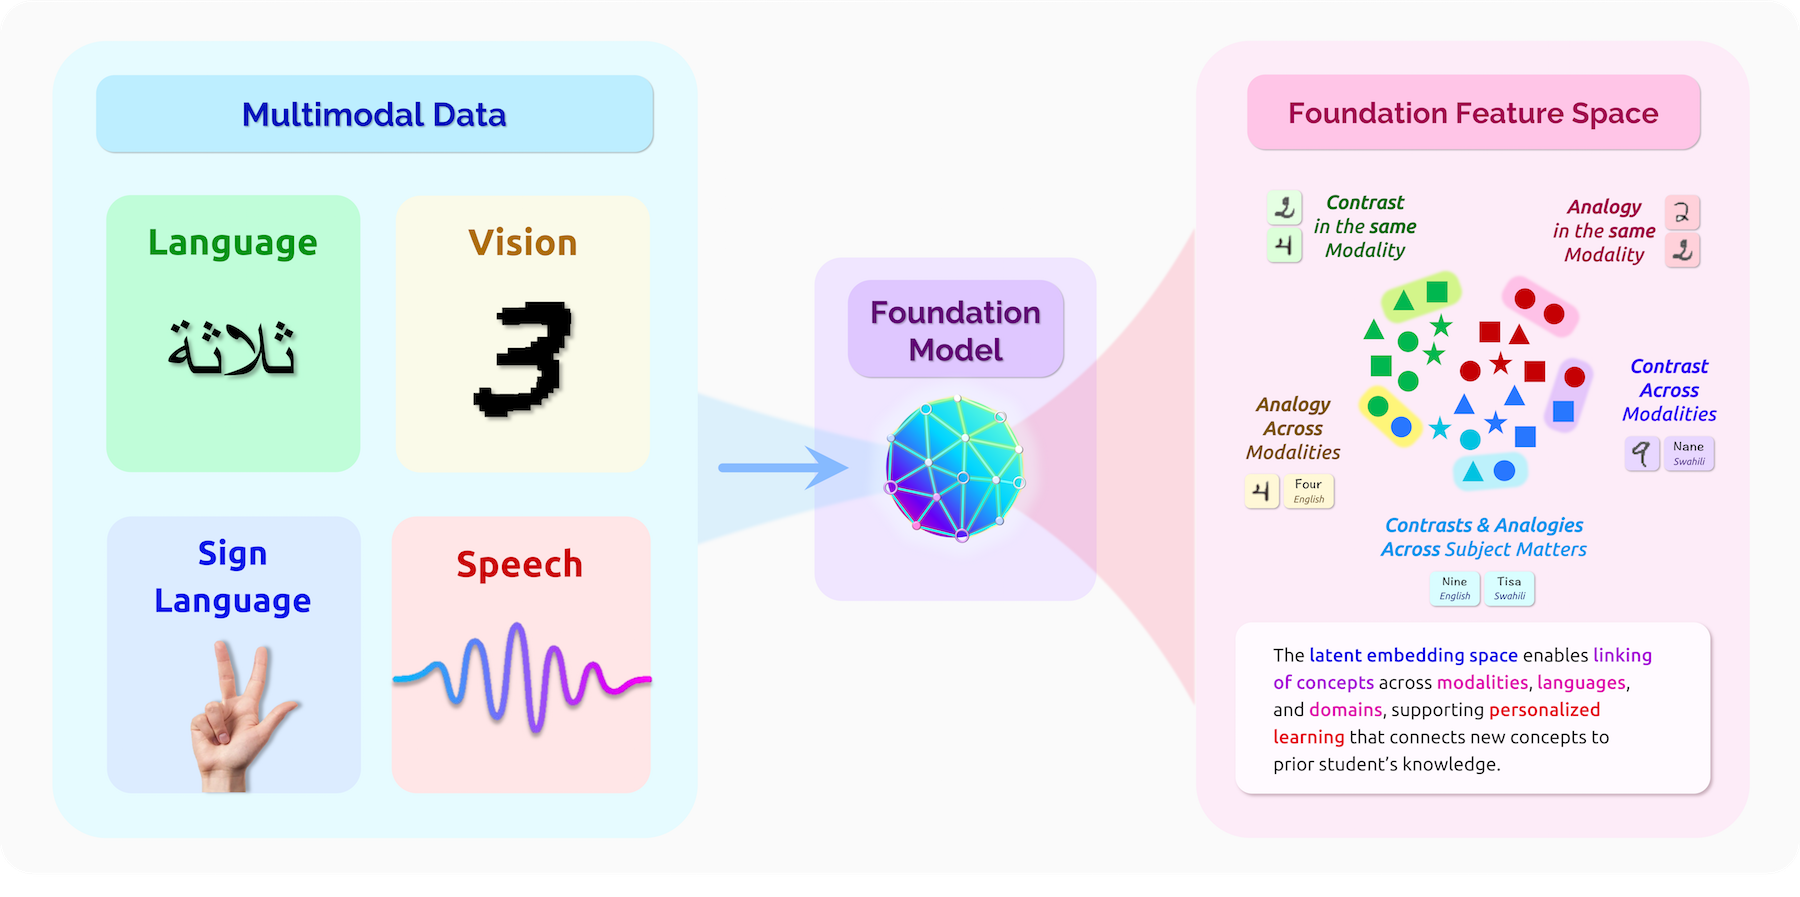
\includegraphics[width=0.88\linewidth]{applications/education_figs/Education_multimodal.png}
% \caption{\dor{TODO: Extend caption}}
% \label{fig:education_multimodal}
% \end{wrapfigure}

\begin{figure}[t]
    \centering
    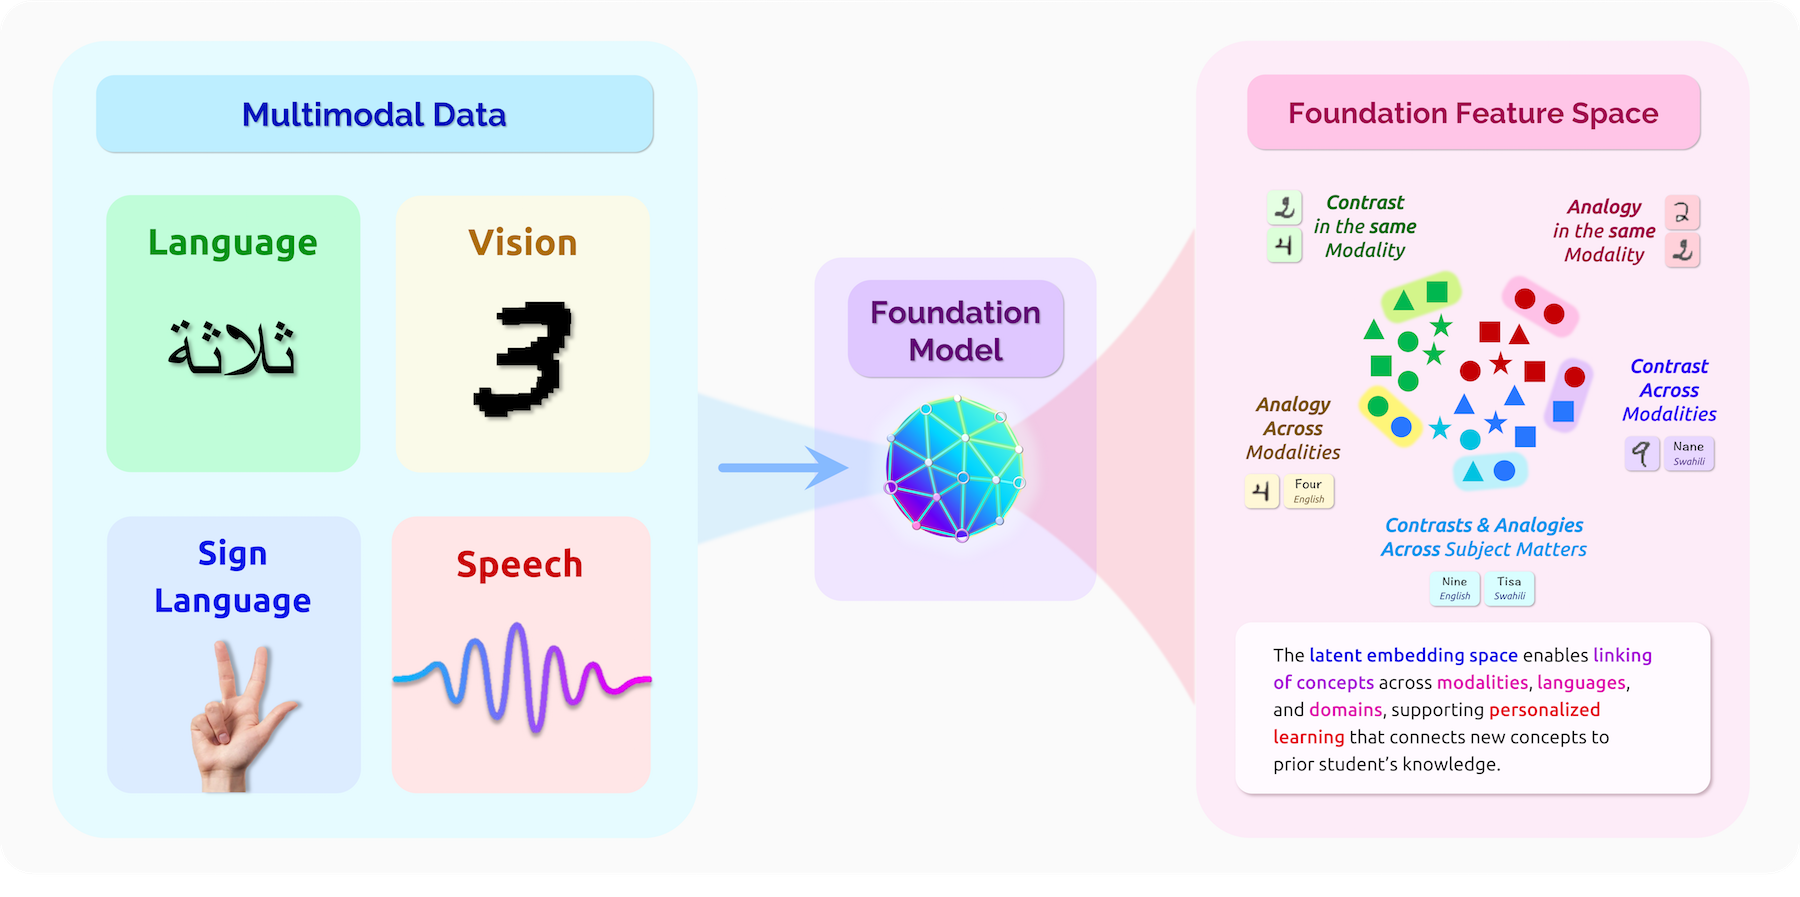
\includegraphics[width=\linewidth]{applications/education_figs/Education_multimodal.png}
    \caption{The figure illustrates a system that embeds signals from various modalities (image, speech, sign, text) and languages into a universal feature space. Such a feature space allows ideas to be linked across modalities and languages. Pedagogically relevant link types include analogies (similarities across languages) and contrasts (distinct concepts across languages), both of which can occur in the same modality or across different modalities.}
    % \pl{I don't get the analogies and contrasts, and why 'languages' is important here if we're talking about education in general}\dora{+1, I think a figure where the reader can immediately see the link to education might be more appropriate here}}
    \label{fig:education_mm}
\end{figure}

Many of the issues in \refsec{ethics} apply to education. For example, as in many other domains, small biases in foundation model training data could be hard to track down \cite{dixon2018bias, bolukbasi2016}, but have important implications for equity of educational access. Moreover, these systems may experience a high degree of ``feedback", where the collected data continually reinforces the model's decisions. 
This issue of bias goes beyond what data is collected and includes concerns over the applications that researchers choose to work on. 
Below, we discuss other education-specific  issues.
% Perhaps AI of the future will allow the already highly resourced students to gain extra educational advantages. Beyond the classic challenges of AI applications, there are a few education specific ideas worth mentioning.
% \refsec{inequality}.




\paragraph{Privacy and security.} One important ethical issue in the use of AI in education is highlighted by the strict legal guidelines concerning privacy in student work. For example, in the United States, student information is protected by the Family Education Rights and Privacy Act (FERPA). These laws and regulations are especially important for children under 13, who have their data privacy and security additionally protected by the Children's Online Privacy Protection Act. Among other things, FERPA limits teachers from sharing personally identifiable student work. This could directly impact initiatives to share data used both for training and for evaluating foundation models. Moreover, there is an open question as to whether the weights of a foundation model could somehow leak the (possibly private) data it was trained upon \cite{nasrPrivacy2018, songRemember2017}. These issues, and their corresponding approaches, are similar to the challenges described in  \refsec{healthcare}. 

\paragraph{The impact of fewer teachers.} One of the goals of digital education, especially based on AI, is to increase the \emph{productivity} of the learning experience so that more learning happens per unit time or unit cost. One can imagine that decision makers could use this increased productivity to remove human teachers from the loop. The long term implications of such decisions are hard to know \emph{a priori}. Could interacting with an education system optimized to maximize ``learning'' have adverse effects on socioemotional skill development? Could it create fewer opportunities for interacting with others? Loneliness is on the rise in younger generations \citep{cigna_2018}, and teachers could be a modulating force for pressures that AI researchers might not envision.

% Many algorithms used to help students can be used to augment human instructors. Similarly there is an exciting line of research to provide feedback to teachers as they instruct\dash{}in much the same way that we would provide feedback to students as they solve open-ended challenges.

\paragraph{Students using foundation-model-based tools.} Another challenge is how to effectively teach students who have access to foundation-model-based tools. For example, it will be much more complex for teachers to understand the extent of a student's contribution if the student worked together with a powerful generative model, or to regulate ineffective collaborations and detect plagiarism. Visual Studio has recently released GitHub CoPilot, an AI pair-programmer built upon GPT-3 \cite{chen2021evaluating}. How will this change computer science education? Many challenges for beginner programmers might be trivial to CoPilot or its technical successors, which could undermine the learning experience for novices. It would be instructive to study other examples of technological advances that disrupted education for certain subjects, such as calculators in math classrooms and Google Translate in language courses, both of which now coexist with traditional instruction.

% There are many other important questions such as: who will own AI for education tools? 
% Will the foundation models adapted for education be publicly owned?
% Will the tools built on top of foundation models be free to use?
% The ideas in this short section are by no means exhaustive.  

% Given that education is a fundamental component of society, research into these issues as well as a critical exploration into currently-unknown risks, should be undertaken as soon as possible.
% \pl{This sentence doesn't add that much value...could just cut or elaborate; in general, I'd avoid one-sentence paragraphs} \pw{+1 for cutting}

% \pl{Besides sharpening this section (more specificity to foundation models, more citations, more authoritative on the education front), the biggest thing I see that's missing is talking about the data that's used to train the foundation model - is it education specific? Most of this seems to just assume a magic foundation model exist, but do we need an education-specific foundation model or could we even train one?}

